\documentclass[a4paper,11pt]{scrartcl}
\usepackage[utf8]{inputenc}
\usepackage[english]{babel}

\usepackage[headsepline]{scrlayer-scrpage}
\ihead{Bernd Schwarzenbacher}
\chead{CMSDE HW3}
\ohead{\today}

\usepackage{siunitx}
\usepackage{amsmath}
\usepackage{amssymb}
\usepackage{commath}
\usepackage[retainorgcmds]{IEEEtrantools}

\usepackage{hyperref}
\usepackage[noabbrev]{cleveref}
\usepackage{graphicx}
\usepackage{listings}

\newcommand*{\E}{\mathbb{E}}
\newcommand*{\EV}[1]{\E\left[{#1}\right]}
\newcommand*{\Var}[1]{\text{Var}\left({#1}\right)}

\newcommand*{\dt}{\dif{}t}
\newcommand*{\Dt}{\Delta{}t}
\newcommand*{\ds}{\dif{}s}
\newcommand*{\dW}{\dif{}W}
\newcommand*{\DW}{\Delta{}W}
\newcommand*{\dX}{\dif{}X(t)}

\newcommand*{\Xb}{\bar{X}}

\usepackage{enumitem}

\begin{document}

\begin{enumerate}

\item
    The geometric Brownian motion
    \[ S(T) = S_0 \exp\left(\left(r-\frac{\sigma^2}{2}\right)T + \sigma W(T)\right)\]
    fulfills the SDE
    \begin{IEEEeqnarray*}{rCl}
      \dif{}S(t) &=& r S(t) \dif{}t + \sigma S(t) \dif{}W(t)  \\
      S(0) &=& S_0
    \end{IEEEeqnarray*}

\begin{enumerate}[leftmargin=1em]
  \item
    The price of a European call option is
    \[ f(0, S_0) = e^{-rT} \EV{\max{(S(T) - K, 0)\left|S(0) = S_0 \right.}} = e^{-rT} \EV{g(0, S_0)}\]
    I apply a Monte Carlo method to compute an approximation $\bar{g}(0, S_0) \approx g(0, S_0)$.
    To obtain the accuracy for this approximation, I use the central limit theorem
    \[ \frac{\sum^N_i \bar{g}_i}{N} - \mu \rightharpoonup
      \mathcal{N}\left(0, \frac{\sigma^2}{N}\right) \]

    \[ \sigma^2 = \EV{g^2} - \EV{g}^2 = \EV{\left( g - \EV{g} \right)^2}\]
    sample variance:
    \[ \hat{\sigma}^2 = \frac{1}{N - 1} \sum_{i=1}^N \left( \bar{g_i}  -
        \frac{\sum^N_{j=1}  \bar{g}_j}{N} \right)^2 \]

    So for $f$ the variance of its approximation $\bar{f}$ can be computed as
    \[ \Var{\bar{f}} = e^{-2rT} \Var{\bar{g}}\]
    With the central limit theorem the error $\epsilon_N$ tends in distribution
    to:
    \[ \sqrt{N} \epsilon_N \rightharpoonup \mathcal{N}\left( 0, e^{-2rT} \hat{\sigma}^2 \right)\]

  \item
    Compute the sensitivity
    \[ \Delta \equiv \frac{\partial{}f(0,s)}{\partial{}s} \approx
      \frac{f(0,s+\Delta{}s) - f(0,s)}{\Delta{}s}\]

    Plotted in \cref{fig:delta}.
    Better methods maybe adaptive?

\begin{figure}[h]
    \begin{minipage}[b]{.5\linewidth}
      \centering
      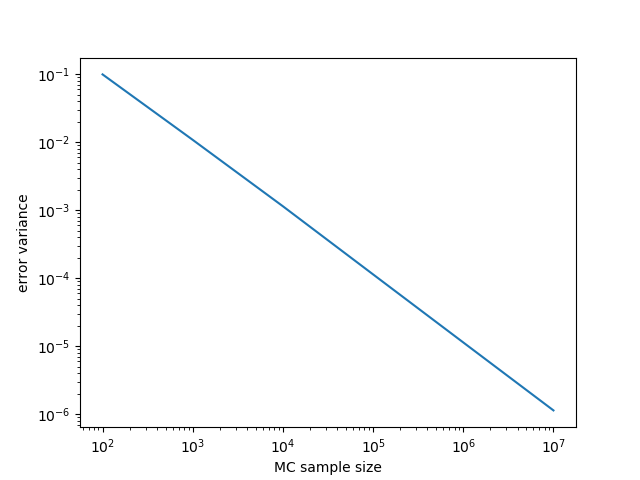
\includegraphics[width=\linewidth]{error_var.png}
      \caption{Error variance}
      \label{fig:error_var}
    \end{minipage}%
    \begin{minipage}[b]{.5\linewidth}
      \centering
      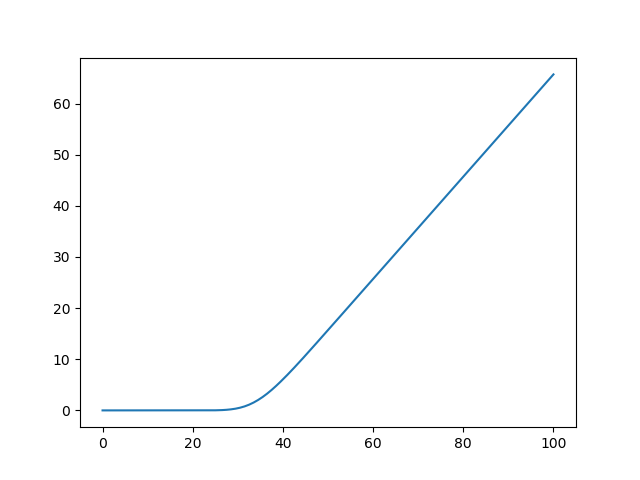
\includegraphics[width=\linewidth]{delta_f.png}
      \caption{Delta}
      \label{fig:delta}
    \end{minipage}
\end{figure}

\end{enumerate}

\item
\begin{enumerate}[leftmargin=1em]
  \item
    Find the solution for the SDE
    \[\dif{}Y(t) = \left( -\alpha (2+Y(t)) + 0.4 \sqrt{\alpha} \sqrt{1-\rho^2}
      \right) \dt + 0.4 \sqrt{\alpha} \dif{}\hat{Z}(t)\]
    with
    \[\hat{Z}(t) = \rho W(t) + \sqrt{1-\rho^2} Z(t)\]
    I use separation of variables to solve this $Y(t) = U(t)V(t)$.
    $U(t)$ solves
    \[ \dif{}U(t) = -\alpha U(t) \dt, U(0)=1\]
    and thus $U(t) = e^{-\alpha t}$.
    $V(t)$ solves
    \[ \dif{}V(t) = \gamma(t)\dt + \theta(t)\dif{}\hat{Z}(t), V(0) = Y(0)\]
    The coefficients $\gamma(t)$ and $\theta(t)$ can be found be comparing
    coefficients in the original equation with the coefficients from applying
    the product rule
    \begin{IEEEeqnarray*}{rCl}
    \dif{}Y(t) &=& \dif{}(U(t)V(t)) = V(t)\dif{}U(t) + U(t)\dif{}V(t) +
    \dif\left<U,V\right>_t \\
    &=& -\alpha Y(t) \dt + U(t) \gamma(t)\dt + U(t) \theta(t)\dif{}\hat{Z}(t)
    \end{IEEEeqnarray*}
    Thus
    \[ \gamma(t) = \frac{-2\alpha+0.4\sqrt{\alpha}\sqrt{1-\rho^2}}{U(t)}, \quad
    \theta(t) = \frac{0.4\sqrt{\alpha}}{U(t)}\]
  and
    \begin{IEEEeqnarray*}{rCl}
  Y(t) &=& U(t)V(t) = e^{-\alpha t} \left( Y_0 + \int_0^t e^{\alpha s}\left(-2\alpha
      + 0.4\sqrt{\alpha}\sqrt{1-\rho^2}\right)\ds + \int_0^t e^{\alpha s} 0.4
      \sqrt{\alpha} \dW(s)\right) \\
  &=& e^{-\alpha t} \left( Y_0 + \left(e^{\alpha t}-1\right)\left(-2
      + \frac{0.4}{\sqrt{\alpha}}\sqrt{1-\rho^2}\right) + \int_0^t e^{\alpha s} 0.4 \sqrt{\alpha} \dW(s)\right)
    \end{IEEEeqnarray*}
    For the expected value of $Y(t)$ I obtain:
    \[ \EV{Y(t)} = e^{-\alpha t}\left(  \EV{Y_0} + \left( e^{\alpha t} -1 \right)
      \left( -2 + \frac{0.4}{\sqrt{\alpha}}\sqrt{1-\rho^2}\right)\right)
      \underset{t\rightarrow\infty}{\longrightarrow} -2 + \frac{0.4}{\sqrt{\alpha}}\sqrt{1-\rho^2}\]
    For the variance, with $\left( e^{\alpha t} - 1 \right)\left( -2 +
      \frac{0.4}{\sqrt{\alpha}}\sqrt{1-\rho^2} \right) = b$:

    \begin{IEEEeqnarray*}{rCl}
      \Var{Y(t)} &=& \EV{Y(t)^2} - \EV{Y(t)}^2 \\
      &=& e^{-2\alpha t} \left(\EV{Y_0^2} + b^2 + \int_0^t e^{2\alpha s} 0.16
        \alpha \dt + 2 \EV{Y_0} b\right)
      - e^{-2\alpha t} \left( \EV{Y_0}^2 + b^2 + 2 \EV{Y_0} b \right) \\
      &=& e^{-2\alpha t} \left( \Var{Y_0} + 0.08 \left( e^{2\alpha t} -
          1\right)\right) \\
      &\underset{t\rightarrow\infty}{\longrightarrow}& 0.08
    \end{IEEEeqnarray*}

  \item
    \[\dX = -\alpha X(t)\dt + \sqrt{\alpha} \dW(t)  \]
  \begin{enumerate}[leftmargin=1em]
    \item
    By separation of variables $X(t) = U(t)V(t)$ I obtain the solution:
    \[ X(t) = e^{-\alpha t} \left( X_0 + \int_0^t e^{\alpha s} \sqrt{\alpha} \dW(s) \right)\]
    Thus the expected value for $X(t)$ is
    \[ \EV{X(t)} = e^{-\alpha t} \EV{X_0} \underset{t\rightarrow\infty}{\longrightarrow} 0\]
    and variance (assuming $X_0$ is independent of $W(t)$)
    \begin{IEEEeqnarray*}{rCl}
      \Var{X(t)} &=& \EV{X(t)^2} - \EV{X(t)}^2 \\
      &=& e^{-2\alpha t}\left(\EV{X_0^2}
      + \EV{2 X_0 \int_0^t e^{\alpha s} \sqrt{\alpha} \dW(s)}
      + \EV{\left(\int_0^t e^{\alpha s} \sqrt{\alpha} \dW(s) \right)^2}\right) \\
      &&- e^{-2\alpha t} \EV{X_0}^2 \\
      &=& e^{-2\alpha t} \left(\EV{X_0^2} + \EV{\int_0^t e^{2\alpha s} \alpha
          \dt} - \EV{X_0}^2\right) \\
      &=& e^{-2\alpha t} \left(\Var{X_0} + \frac{e^{2\alpha t} - 1}{2}  \right)
      = e^{-2\alpha t} \Var{X_0} + \frac{1 - e^{-2\alpha t}}{2}
      \underset{t\rightarrow\infty}{\longrightarrow} \frac{1}{2}
    \end{IEEEeqnarray*}

    \item Forward Euler approximation
      \[\Xb_n = X_0 + \sum_{i=0}^{n-1} -\alpha \Xb_i (t_{i+1} - t_i) +
        \sqrt{\alpha} (W_{i+1} - W_{i})  \]
      \[\Xb_0 = X_0\]
      \[\Xb_i = \Xb_{i-1} - \alpha \Xb_{i-1} (t_i - t_{i-1}) + \sqrt{\alpha}
        (W_i - W_{i-1}) = \Xb_{i-1}(1-\alpha\Dt) + \sqrt{\alpha} \DW_i \]
      \[\EV{\Xb_i} = \EV{\Xb_{i-1}} (1 - \alpha \Dt) = \EV{X_0} (1-\alpha\Dt)^i
      \underset{i\rightarrow\infty}\longrightarrow 0 \]
    \begin{IEEEeqnarray*}{rCl}
      \Var{\Xb_i} &=& \EV{\Xb_i^2} - \EV{\Xb_i}^2 \\
      &=& \EV{\Xb^2_{i-1}(1-\alpha\Dt)^2 + 2 \Xb_{i-1}(1-\alpha\Dt) \sqrt{\alpha}
        \DW_i + \alpha \DW_i^2} - \EV{\Xb_{i-1}}^2(1-\alpha\Dt)^2 \\
      &=& \EV{\Xb^2_{i-1}} (1-\alpha\Dt)^2 + \alpha \Dt -
      \EV{\Xb_{i-1}}^2(1-\alpha\Dt)^2 \\
      &=& \Var{\Xb_{i-1}} (1-\alpha\Dt)^2+ \alpha \Dt \\
      &=& \Var{X_0} (1-\alpha\Dt)^{2(i+1)} + \alpha\Dt\sum_{j=0}^{i-1}
        (1-\alpha\Dt)^{2j} \\
      &=& \Var{X_0} (1-\alpha\Dt)^{2(i+1)} + \alpha\Dt\frac{1 -
        (1-\alpha\Dt)^{2i}}{1-(1-\alpha\Dt)^2} \\
    &\underset{i\rightarrow\infty}{\longrightarrow}&
    \frac{\alpha\Dt}{2\alpha\Dt-(\alpha\Dt)^2} = \frac{1}{2 - \alpha\Dt}\\
    \end{IEEEeqnarray*}

    \item Backward Euler approximation
      \[\Xb_n = X_0 + \sum_{i=0}^{n-1} -\alpha \Xb_{i+1} (t_{i+1} - t_i)
        + \sqrt{\alpha} (W_{i+1} - W_{i}) \]
      \begin{IEEEeqnarray*}{rCl}
        \Xb_i &=& \Xb_{i-1} - \alpha \Xb_i (t_i - t_{i-1}) + \sqrt{\alpha}
        (W_i - W_{i-1}) \\
        &=& \frac{\Xb_{i-1} + \sqrt{\alpha} \DW_i}{1+\alpha\Dt}
      \end{IEEEeqnarray*}

    Expected value:
    \[\EV{\Xb_i} = \frac{\EV{\Xb_{i-1}}}{1+\alpha\Dt} = \EV{X_0}
      (1+\alpha\Dt)^{-i} \underset{i \rightarrow\infty}{\longrightarrow} 0
    \]

    Variance:
    \begin{IEEEeqnarray*}{rCl}
      \Var{\Xb_i} &=& \EV{\Xb_i^2} - \EV{\Xb_i}^2 \\
      &=& \EV{\frac{\Xb_{i-1}^2 + 2 X_{i-1} \sqrt{\alpha}\Dt\DW_i +
          \alpha(\DW_i)^2}{(1+\alpha\Dt)^2}} - \frac{\EV{\Xb_{i-1}}^2}{(1+\alpha\Dt)^2} \\
      &=& \frac{\EV{\Xb_{i-1}^2} + \alpha\Dt - \EV{\Xb_{i-1}}^2}{(1+\alpha\Dt)^2}
      = \frac{\Var{\Xb_{i-1}} + \alpha\Dt}{(1+\alpha\Dt)^2} \\
      &=& \frac{\Var{X_0}}{(1+\alpha\Dt)^{2i}} + \alpha\Dt \sum_{j=1}^{i-1}
      (1+\alpha\Dt)^{-2j} \\
      &=& \frac{\Var{X_0}}{(1+\alpha\Dt)^{2i}} - \alpha\Dt
      + \alpha\Dt\frac{1 - (1+\alpha\Dt)^{-2(i-1)}}{1-(1+\alpha\Dt)^{-2}} \\
      &\underset{i\rightarrow\infty}\longrightarrow& -\alpha\Dt +
      \frac{\alpha\Dt}{1-\frac{1}{(1+\alpha\Dt)^2}} =
      -\alpha\Dt + \frac{\alpha\Dt (1+\alpha\Dt)^2}{(1+\alpha\Dt)^2-1} \\
      &=& -\alpha\Dt + \frac{\alpha\Dt (1+ 2\alpha\Dt +
        (\alpha\Dt)^2)}{2\alpha\Dt + (\alpha\Dt)^2}
      = \frac{-2\alpha\Dt - (\alpha\Dt)^2 + 1 + 2\alpha\Dt +
        (\alpha\Dt)^2}{2+\alpha\Dt} \\
      &=& \frac{1}{2+\alpha\Dt}
    \end{IEEEeqnarray*}

    \item Interpretation:
      Seems like variance is better for forward Euler.
  \end{enumerate}

  \item
    I implemented the following Forward Euler method
    \begin{IEEEeqnarray*}{rCl}
      S_{n+1} - S_n &=& r S_n \Dt + e^{Y_n} S_n \DW_n \\
      Y_{n+1} - Y_n &=& \left(-\alpha(2+Y_n) + 0.4\sqrt{\alpha}
        \sqrt{1-\rho^2}\right) \Dt + 0.4 \sqrt{\alpha} \Delta\hat{Z}_n \\
      \hat{Z}_n &=& \rho W_n + \sqrt{1-\rho^2} Z_n
    \end{IEEEeqnarray*}

    The parameters used where $\alpha=100, r=0.04, T=\frac{3}{4}, Y_0 = -1,
    S_0=K=100$ and $\rho=-0.3$.

    With \num{e4} Monte Carlo samples and \num{e3} equidistant time steps I
    get for the option value
    \[ e^{-rT} \EV{\max{(S(T) - K, 0)}} = \num{6.92}\]
    % The code can be found in \cref{lst:ex2}.

  \item
\end{enumerate}

\end{enumerate}

% \section{Code Appendix}

% All code can be found online at
% \url{https://github.com/bschwb/cmsde/tree/master/hw3}

% \begin{listings}
%   \lstinputlisting{exercise2.py}
% \end{listings}

\end{document}